\documentclass[thesis.tex]{subfiles}

\begin{document}

\iffulldocument\else
	\chapter{KdV5}
\fi

\section{Overview}

A periodic multi-pulse is a multi-modal solution to \cref{eqODE} on a periodic domain. Heuristically, we construct a periodic multi-pulse by gluing together multiple copies of the primary pulse end-to-end in a loop as shown in \cref{fig:permultipulse}.
\begin{figure}
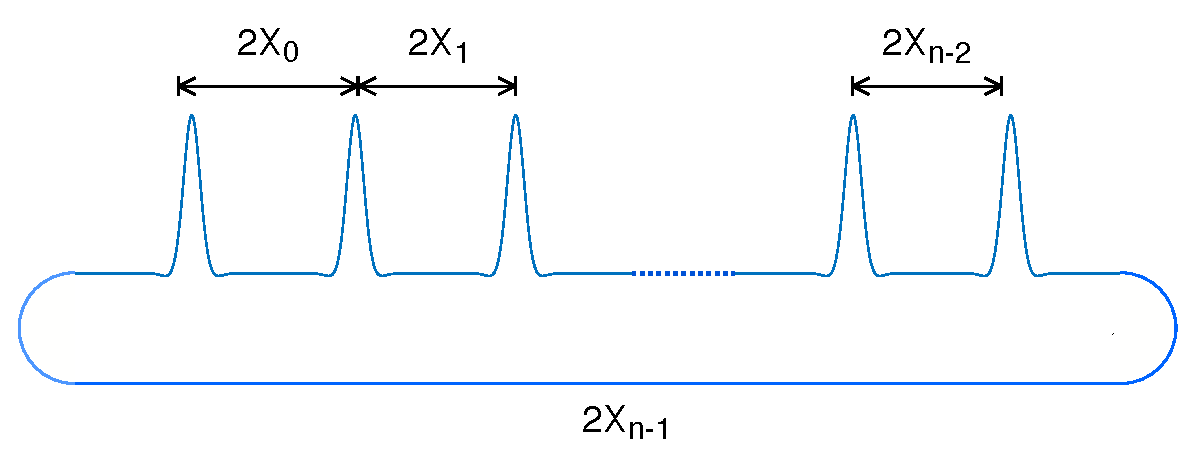
\includegraphics[width=10cm]{periodic/multipulseperiodic}
\caption{Periodic $n-$pulse solution.}
\label{fig:permultipulse}
\end{figure}

In this chapter, we will start by proving the existence periodic multi-pulses. We will exhibit a bifurcation structure for periodic 2-pulses. We will then look at their spectral stability.

\section{Existence}

First, we will look at existence. From a spatial dynamics perspective, a periodic multi-pulse is a multi-loop periodic orbit solution $Q_n(x)$ to
\begin{equation}\label{existgenODE}
U'(x) = F(U(x); c)
\end{equation}
which remains close to the primary homoclinic orbit $Q(x)$. A periodic $n$-pulse can be described by $n$ pulse distances $\{X_0, \dots, X_{n-1} \}$, where the distance between consecutive copies of $Q(x)$ in the loop is $2 X_j$. The period of the orbit is $2X$, where $X = X_0 + \dots + X_{n-1}$. A periodic $n$-pulse requires one more pulse distance than an $n$-homoclinic orbit, since we need one more connection to ``close the loop''.  

From a mathematical perspective, rather than describing a periodic multi-pulse by its pulse distances $X_j$, we will adopt an alternative parameterization which is both more convenient and captures the underlying geometry necessary for a periodic $n$-pulse to exist. This parameterization is an adaptation of that in \cite{SandstedeStrut,Sandstede1998} to the periodic case. 

From Hypothesis \ref{hypeqhyp}, the rest state at 0 is a hyperbolic equilibrium point of \cref{existgenODE}. The linearization $DF(0; c)$ about the rest state has a quartet of eigenvalues $\pm \alpha_0 \pm \beta_0 i$. All other eigenvalues have real part strictly larger in magnitude than $\alpha_0$. Let
\begin{equation}\label{defrho}
\rho = \frac{\beta_0}{\alpha_0}
\end{equation}
and
\begin{equation}\label{pstar}
p^* = \arctan \rho.
\end{equation}
Define the set
\begin{align}
\mathcal{R} &= \left\{ \exp\left(-\frac{2 k \pi}{\rho}\right) : k \in \N_0 \right\} \cup \{ 0 \},
\end{align}
which is a complete metric space. We will use $r \in \mathcal{R}$ as a scaling parameter. The parameterization is defined as follows.

\begin{definition}\label{def:perparam}
For $n \geq 2$, a \emph{periodic parameterization} of a periodic $n$-pulse is a sequence of parameters $(m_0, \dots, m_{n-1}, \theta)$, where
\begin{enumerate}[(i)]
\item $m_j$ is a nonnegative integer, with at least one of the $m_j \in \{0, 1\}$.
\item $\theta \in [-p^*, \pi - p^*)$.
\end{enumerate}
\end{definition}

The physical pulse distances $X_j$ are determined by these parameters and by the scaling parameter $r$. If $r = \exp\left(-\frac{2 m \pi}{\rho}\right)$, then
\[
X_j \approx \frac{\pi}{2 \beta_0}(2 m + m_j) + L_0
\]
where $L_0$ is a constant. [PUT A NICE PICTURE HERE OF WHAT THE $m_j$ and $r$ MEAN PHYSICALLY.] 

We can now state the main theorem of this section, which gives conditions for the existence of periodic multi-pulses. The requirement that the scaling parameter $r$ be sufficiently small means that the individual pulses must be well-separated. 

\begin{theorem}[Existence of $n$-periodic solutions]\label{perexist}
Assume Hypotheses \ref{Ehyp}, \ref{Hhyp}, \ref{hypeqhyp}, \ref{Qexistshyp}, and \ref{H0transversehyp}. Let $Q(x)$ be the transversely constructed, symmetric primary pulse solution to \eqref{genODE} from Hypothesis \ref{Qexistshyp}. For any periodic parameterization $(m_0, \dots, m_{n-1}, \theta)$ with $\theta \notin \{-p^*, \pi - p^*) \}$, there exists $r_* \in \mathcal{R}$ with $r_* > 0$ such that for any $r \in \mathcal{R}$ with $r \leq r_*$:
\begin{enumerate}[(i)]
	\item There exists a periodic $n$-pulse solution $Q_n(x; m_0, \dots, m_{n-1}, \theta, r)$ to \eqref{genODE}.

	\item The distances between consecutive copies of $Q(x)$ are
	\begin{align}\label{Xj}
		X_j(r; m_j, \theta) &= \frac{1}{2 \alpha_0} |\log r| + \frac{\pi}{2\beta_0} b_j(r; m_j, \theta) + L_0 && j = 0, \dots, n-1,
	\end{align}
	where the $b_j(r; m_j, \theta): \mathcal{R} \rightarrow \R$ are smooth functions with $b_j(0; m_j, 0) = m_j$, and $L_0$ is a constant. If $r = \exp\left(-\frac{2 m \pi}{\rho}\right)$, then
	\begin{equation}\label{Xjr}
		X_j(r; m_j, \theta) = \frac{\pi}{2\beta_0}\left( 2m + b_j(r; m_j, \theta) \right) + L_0,
	\end{equation}	

	\item The periodic domain has length $2X$, where
	\begin{align}\label{Xdomain}
	X(r; m_0, \dots, m_{n-1}, \theta) = \frac{n}{2\alpha_0} |\log r| + \frac{\pi}{2\beta_0} \sum_{j=0}^{n-1} b_j(r; m_j, \theta) + n L_0
	\end{align}

	\item $Q_n(x)$ can be written as piecewise perturbation of the primary pulse $Q(x)$. Details are given below in Lemma \ref{solvewithjumps}.
\end{enumerate}
\end{theorem}

\begin{remark}
The periodic $n$-pulses constructed in \cref{perexist} are unique up to ``rotation'' of the integers $(m_0, \dots, m_{n-1})$ in the periodic parameterization. For example, $(m_0, m_1, m_2, \theta)$, $(m_2, m_0, m_1, \theta)$, and $(m_1, m_2, m_0, \theta)$ all give the same solution.
\end{remark}

The condition that $\theta \notin \{-p^*, \pi - p^*) \}$ in \cref{perexist} is used to avoid any bifurcation points which may arise in the construction. For periodic 2-pulses, we can use a symmetry argument to give a complete bifurcation picture. In the next theorem, we state an existence result for periodic 2-pulses and show that asymmetric solutions bifurcate from symmetric solutions in a series of pitchfork bifurcations. We note that we are using a different phase parameter than in \cref{perexist}.

\begin{theorem}\label{2pulsebifurcation}
Assume Hypotheses \ref{Ehyp}, \ref{Hhyp}, \ref{hypeqhyp}, \ref{Qexistshyp}, and \ref{H0transversehyp}. Let $Q(x)$ be a transversely constructed, symmetric primary pulse solution to \eqref{genODE}.

For any positive integer $N$, there exists $r_* \in \mathcal{R}$ with $r_* > 0$ such that for all $r \leq r_*$ and $m_0 \in \{0, 1\}$
\begin{enumerate}[(i)]
	\item There exists a family of symmetric periodic 2-pulses $Q_2(x; m_0, s_0, r)$ parameterized by $s_0 \in [0, \pi)$. The distances $X_j$ are given by
	\begin{equation*}
		X_0(r, s_0) = X_1(r, s_0) = \frac{1}{2 \alpha_0} |\log r| + \frac{\pi}{2\beta_0} (m_0 + s_0) + L_0.
	\end{equation*}
	\item There exists a family of asymmetric periodic 2-pulses $\tilde{Q}_2(x; m_0, s_1, r)$ with distances $\tilde{X}_1 > \tilde{X}_0$ parameterized by $s_1 \in [-p^*, N \pi]$. The distances $\tilde{X}_j$ are given by
	\begin{equation*}
	\begin{aligned}
		\tilde{X}_0(r, s_1) &= \frac{1}{2 \alpha_0} |\log r| + \frac{\pi}{2\beta_0} b_0(r; m_0, s_1) + L_0 \\
		\tilde{X}_1(r, s_1) &= \frac{1}{2 \alpha_0} |\log r| + \frac{\pi}{2\beta_0} s_1 + L_0, 
	\end{aligned}
	\end{equation*}
	where $b_0(r; m_0, s_1)$ is smooth in both $r$ and $s_1$, and $b_0(0; m_0, k \pi) = m_0$ for integers $k = 0, \dots, N$.

	\item The two families meet at a pitchfork bifurcation. In terms of the two parameterizations, this occurs when $s_0 = p^*(r)$ and $s_1 = -p^*$. The bifurcation point $p^*(r)$ is smooth in $r$, and
	\[
	p^*(r)\rightarrow \arctan \rho \text{ as }r \rightarrow 0.
	\]
\end{enumerate}
\end{theorem}
[THIS NEEDS A NICE PICTURE.]

\section{Spectral stability}

In this section, we look at the spectral stability of the periodic multi-pulses which we constructed in the previous section. To do this, we will adapt framework we set up in \cref{sec:genspectrum}.

Let $Q(x)$ be the primary pulse solution. Let $Q_n(x)$ be any periodic multi-pulse solution constructed according to Theorem \ref{perexist}, and let $q_n(x)$ be the first component of $Q_n(x)$. We are interested in the PDE eigenvalue problem
\begin{equation}\label{genPDEeigper}
\partial_x \calL(q_n) v = \lambda v
\end{equation}
resulting from the linearization of the original PDE \cref{genPDE} about $q_n(x)$. From the construction in Theorem \ref{perexist}, it is natural to pose \cref{genPDEeigper} on the space of periodic functions $H^{2m}_{\text{per}}[-X,X]$, where
\[
H^{2m}_{\text{per}}[-X,X] = \left\{ f \in H^{2m}(\R) : f^{(k)}(-X) = f^{(k)}(X) \text{ for } k = 0, \dots, 2m \right\} 
\]
The norm on this space is the $H^{2m}$ norm restricted to $[-X, X]$. 

As in \cref{sec:genspectrum}, we use a spatial dynamics formulation and write the PDE eigenvalue problem \cref{genPDEeigper} as the first order system of ODEs
\begin{equation}\label{PDEeigsystemper2}
\begin{aligned}
V'(x) &= A(Q_n(x))V(x) + \lambda B V(x) \\
V(-X) &= V(X)
\end{aligned}
\end{equation}
where $V(x) \in C^0(\R)$, and we have imposed an additional periodic constraint on $V(x)$. To aid in the analysis, we rewrite \cref{PDEeigsystemper2} as
\begin{equation}\label{PDEeigsystemper3}
\begin{aligned}
V'(x) &= A(Q_n(x); \lambda)V \\
V(-X) &= V(X),
\end{aligned}
\end{equation}
where $A(Q_n(x); \lambda) = A(Q_n(x)) + \lambda B$. Let $A(\lambda) = A(0; \lambda)$. By Lemma \ref{eigA0lemma}, $A(0)$ has a simple eigenvalue at 0. The next lemma states that for small $\lambda$, $A(0)$ has a simple eigenvalue $\nu(\lambda)$ near 0.

% nu(lambda) lemma
\begin{lemma}\label{nulambdalemmasimple}
There exists $\delta_0 > 0$ such that for $|\lambda| < \delta_0$, the matrix $A(\lambda)$ has a simple eigenvalue $\nu(\lambda)$ near 0.
\begin{proof}
This is proved as part of Lemma \ref{nulambdalemma} below.
\end{proof}
\end{lemma}

We can now state the main theorem of this section, which provides a condition for \cref{PDEeigsystemper3} to have solution for a particular $\lambda$. Since the spatial dynamics formulation \cref{PDEeigsystemper3} is equivalent to the PDE eigenvalue problem, this allow us to find the eigenvalues of \cref{genPDEeigper}. This theorem is analogous to \cite[Theorem 2]{Sandstede1998}, where the matrix $S(\lambda)$ is replaced by a block matrix.

% block matrix theorem
\begin{theorem}\label{blockmatrixtheorem}
Assume Hypotheses \ref{Ehyp}, \ref{Hhyp}, \ref{hypeqhyp}, \ref{Qexistshyp}, and \ref{H0transversehyp}, and \ref{Melnikov2hyp}. Let $Q(x)$ be the primary pulse solution, and let $\Psi(x)$ be the solution to the adjoint variational equation from Lemma \ref{varadjsolutions}. Choose any periodic parameterization $(m_0, \dots, m_{n-1}, \theta)$ with $\theta \neq \pm \pi$, and let $r_*$ be as in \cref{perexist}. 

Choose any positive integer $N$. Then for any $r \leq r_*$ there exists $\delta(r,N)$, where $0 < \delta(r,N) < N/|\log r|$, with the following property. There exists a bounded, nonzero solution $V(x)$ of \cref{PDEeigsystemper3} for $|\lambda| < \delta(r,N)$ if and only if
\begin{equation}\label{blockmatrixcond}
E(\lambda) = \det S(\lambda) = 0.
\end{equation}
$S(\lambda)$ is the $(2n \times 2n)$ block matrix
\begin{equation}\label{blockeq}
S(\lambda) = 
\begin{pmatrix}
K(\lambda) + C_1 & \lambda K_1(\lambda) + D_1 \\
-\lambda M^c K^+(\lambda) C_2 & A - \lambda^2 MI + D_2
\end{pmatrix}
\end{equation}
The individual terms in $S(\lambda)$ are as follows.

\begin{enumerate}
\item $K(\lambda)$ is the banded matrix
\begin{equation}
K(\lambda) = 
\begin{pmatrix}
e^{-\nu(\lambda)X_1} & & & & & -e^{\nu(\lambda)X_0} \\
-e^{\nu(\lambda)X_1} & e^{-\nu(\lambda)X_2} \\
& -e^{\nu(\lambda)X_2} & e^{-\nu(\lambda)X_3} \\
& \ddots & \ddots & &&  \\
& & & & -e^{\nu(\lambda)X_{n-1}} & e^{-\nu(\lambda)X_0} 
\end{pmatrix}
\end{equation}
where $\nu(\lambda)$ is defined in Lemma \ref{nulambdalemmasimple}. $K^+(\lambda)$ is the same matrix with all terms positive.

\item $A$ is the symmetric banded matrix
\begin{align}\label{Asymm}
A &= \begin{pmatrix}
-a_0 -a_1 & a_0 + a_1 \\
a_0 + a_1 & -a_0 - a_1
\end{pmatrix} && n = 2 \\
A &= \begin{pmatrix}
-a_{n-1} - a_0 & a_0 & & &  & a_{n-1}\\
a_0 & -a_0 - a_1 &  a_1 \\
& a_1 & -a_1 - a_2 &  a_2 \\
& \ddots & \ddots & \ddots \\
a_{n-1} & & & & a_{n-2} & -a_{n-2} - a_{n-1} \\
\end{pmatrix} && n > 2 \nonumber
\end{align}
where
\begin{align*}
a_i &= \langle \Psi(X_i), Q'(-X_i) \rangle
\end{align*}

\item $K_1(\lambda)$ is the matrix
\begin{align*}
K_1(\lambda) &= \begin{pmatrix}
s_0^+ - s_1^- & s_1^- &&& -s_0^+ \\
-s_1^+ & s_1^+ - s_2^- & s_2^- \\
& -s_2^+ & s_2^+ - s_3^- & s_3^- \\ && \ddots \\
\\
s_0^- &&& -s_{n-1}^+ & s_{n-1}^+ - s_0^- 
\end{pmatrix}
\end{align*}
with entries
\begin{align*}
s_i^- &= e^{-\nu(\lambda)X_i} q(X_i)\\
s_i^+ &= e^{\nu(\lambda)X_i} q(X_i)\\
\end{align*}
where $q(x)$ is the first component of the primary pulse solution $Q(x)$. 

\item $M$ and $M^c$ are the Melnikov-type integrals
\begin{align*}
M &= \int_{-\infty}^\infty q(y) \partial_c q(y) dy \\
M^c &= \int_{0}^\infty q(y) v^c(y) dy
\end{align*}
where $v^c(y)$ is the first component of $V^c(y)$, which is defined in \cref{varadjsolutions}.

\item The remainder matrices and $K_1(\lambda)$ are analytic in $\lambda$ and have uniform bounds
\begin{align*}
|K_1(\lambda)| &\leq C r^{1/2} \\
|C_1| &\leq C |\lambda|(|\lambda| + r^{1/2}) \\
|D_1| &\leq C |\lambda|(|\lambda| + r^{1/2})^2 \\
|C_2| &\leq C (|\lambda| + r^{1/2})^2 \\
|D_2| &\leq C (|\lambda| + r^{1/2})^3 
\end{align*}
\end{enumerate}
\end{theorem}

To leading order, \cref{blockeq} is block diagonal with blocks $A - \lambda^2 MI$ and $K(\lambda)$. As in \cref{chapter:kdv5homoclinic}, we expect that points where $A - \lambda^2 MI$ is singular will give us interaction eigenvalues as well as two kernel eigenvalues. We will show below that $K(\lambda)$ is singular near the discrete set of points
\begin{align*}
\lambda &= c\frac{k \pi i}{X} && k \in \Z
\end{align*}
We expect that this will give us a set of discrete, purely imaginary eigenvalues (which will include one more kernel eigenvalue). Since these are the periodic analogue of the essential spectrum in the $n$-homoclinic case, we will refer to these as essential spectrum eigenvalues, even though they are technically still part of the point spectrum. 

\begin{remark}
For any positive integer $N$ we choose, it follows from \cref{Xdomain} that for all $r \leq r_*$,
\begin{align*}
\left| c\frac{k \pi i}{X} \right| \leq \delta(r,N) && k \in \Z, |k|\leq N.
\end{align*}
Thus we can use \cref{blockmatrixtheorem} to find the first $N$ essential spectrum eigenvalues.
\end{remark}

\section{Spectrum of periodic 2-pulse}

In this section, we will consider the simplest case, which is the periodic 2-pulse. For this case, $S(\lambda)$ from \cref{blockmatrixtheorem} is a $4\times4$ matrix. With the aid of Mathematica, we can compute its determinant.

\begin{corollary}\label{2blockmatrix}
$E(\lambda)$ from \cref{blockmatrixtheorem} is given by
\begin{equation}\label{2detBeq}
\begin{aligned}
E(\lambda) &= \left(-2 \lambda^2 M (2a + \lambda^2 M) + R_1 \right) \sinh(\nu(\lambda)X) \\
&-4 M M^c \lambda^4 ( q(X_0) \sinh(\nu(\lambda)X_0) + q(X_1) \sinh(\nu(\lambda)X_1) ) \cosh(\nu(\lambda)X)  + R_2
\end{aligned}
\end{equation}
where
\begin{equation}\label{2pa}
a = \langle \Psi(X_0), Q'(-X_0) \rangle + \langle \Psi(X_1), Q'(-X_1) \rangle
\end{equation}
and the remainder terms have bounds
\begin{align*}
|R_1| \leq C(r^{1/2} + |\lambda|)^5 \\
|R_2| \leq C(r^{1/2} + |\lambda|)^6
\end{align*}
\end{corollary}

The interaction eigenvalue pattern will be determined by the quantity $a$ in \cref{2pa}. We characterize this in the next lemma.

\begin{lemma}\label{lemma:chara}
For any positive integer $N$, let $r_*$ be as in Theorem \ref{2pulsebifurcation}. Then for any $r \leq r_*$:
\begin{enumerate}[(i)]
	\item For a symmetric periodic 2-pulse $Q_2(x; m_0, s_0, r)$, $a = r \tilde{a}(r; m_0, s_0)$, where for $m_0 = 0$,
	\begin{equation}
	\begin{aligned}
	\tilde{a}(0; m_0, s_0) &= 0 && \text{if }s_0 = p^* \\
	\tilde{a}(0; m_0, s_0) &> 0 && \text{if }s_0 < p^* \\
	\tilde{a}(0; m_0, s_0) &< 0 && \text{if }s_0 > p^*
	\end{aligned}
	\end{equation}
	These are reversed for $m_0 = 1$.
	\item For an asymmetric periodic 2-pulse $Q_2(x; m_0, s_1, r)$, $a = r \tilde{a}(r; m_0, s_1)$, where for all $s_1 > -p^*$,
	\begin{equation}
	\begin{aligned}
	\tilde{a}(0; m_0, s_1) &> 0 && \text{if }m_0 = 0 \\
	\tilde{a}(0; m_0, s_1) &< 0 && \text{if }m_0 = 1
	\end{aligned}
	\end{equation}
\end{enumerate}
\end{lemma}

We are interested in two parameter regimes. First, we will consider the case where $r$ is sufficiently small so the interaction eigenvalues ``out of the way'' of the essential spectrum eigenvalues. 








\iffulldocument\else
	\bibliographystyle{amsalpha}
	\bibliography{thesis.bib}
\fi

\end{document}